\documentclass[../BTL.tex]{subfiles}
\usepackage{caption}
\usepackage{float}
\usepackage{graphicx}
\begin{document}
Chương 2 đã trình bày về....Chương 3 này chúng em sẽ trình bày chi tiết về cách xây dựng, đánh giá mô hình và kết quả thực nghiệm thu được.
%mô tả tập dữ liệu
\section{Sơ đồ phương pháp phân loại}
Trong bài tập lớn này, màu sắc được phân loại bằng cách sử dụng thuật toán phân loại Machine Learning K-Nearest Neighbors. Mô hình phân loại này được huấn luyện bởi các giá trị biểu đồ màu R, G, B của hình ảnh. Quá trình thực hiện được mô tả bằng hình dưới đây

Cụ thể:

\section{Mô tả tập dữ liêu}
Tập dữ liệu của mô hình bao gồm 2 loại: tập Training, tập Test. Tập Training gồm 5053 mẫu dữ liệu được chia làm 11 màu: đen, xanh dương, xanh lá, nâu, xám, cam, hồng, tím, đỏ, trắng và vàng được mô tả cụ thể trong hình \ref{fig: data_training}. Tập Test gồm 307 mẫu dữ liệu với đầy đủ 11 màu kể trên. Mỗi mẫu dữ liệu trong bài toán là một hình ảnh được phân tích theo biểu đồ màu RGB thành 3 đặc trưng và 1 nhãn, cụ thể trong hình \ref{fig:data}. Tập Training được sử dụng để huấn luyện mô hình còn tập Test được sử dụng để đánh giá độ chính xác sau khi huấn luyện
\begin{figure}[h]
    \centering
    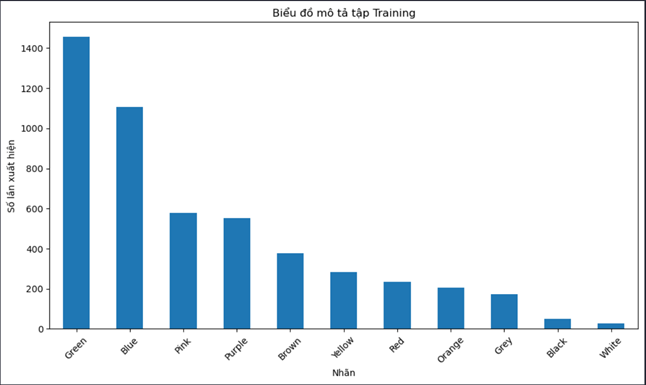
\includegraphics[scale = 0.85]{BTL BaoCao Latex TTNT/Anh/mô tả tập Training.png}
    \caption{Biểu đồ mô tả tập dữ liệu training}
    \captionsetup{justification=centering}
    \label{fig: data_training}
\end{figure}
\hfill
\begin{figure}[H]
    \centering
    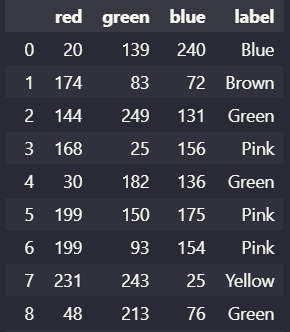
\includegraphics[scale=0.8]{BTL BaoCao Latex TTNT/Anh/data.png}
    \caption{Dữ liệu Training/Test}
    \label{fig:data}
\end{figure}

%trích xuất đặc trưng
\section{Tiền xử lý dữ liệu}
Như đã nêu ở phần trước, mô hình này sử dụng biểu đồ màu RGB để trích xuất các đặc trưng màu sắc của ảnh. 
\subsection{Khai báo các thư viện}
Thư viện os: được sử dụng trong quá trình duyệt từng tệp trong thư mục.

Thư viện cv2: được sử dụng trong quá trình xử lý ảnh

Thư viện numpy: được sử dụng để tính toán số học và ma trận

\begin{figure}[H]
    \centering
    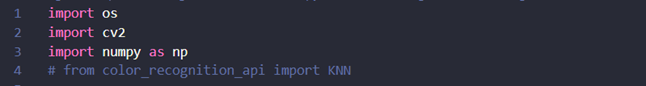
\includegraphics[scale=0.6]{BTL BaoCao Latex TTNT/Anh/thư viện để trích xuất đặc trưng.png}
    \caption{Khai báo các thư viện cần thiết khi trích xuất đặc trưng màu ảnh}
    \captionsetup{justification=centering}
    \label{fig:color_feagure}
\end{figure}

\subsection{Xây dựng hàm}
\subsubsection{Đối với mẫu dữ liệu Training/Test}
Để lấy các đặc trưng về màu sắc của ảnh, ta sử  hàm color\_histogram\_of\_imag để tính toán các histogram của 1 ảnh tên img\_nam theo biểu đồ màu RGB, sau đó đặc trưng của mẫu dữ liệu sẽ được ghi vào tệp testing.data cùng với nhãn mô tả. 

Để đọc ảnh từ máy, tách ảnh thành các kênh màu B, G, R và tính toán các histogram của các kênh màu, ta sử dụng các hàm trong thư viện OpenCV. Nhãn của mẫu dữ liệu được gán theo tên thư mục đang chứa mẫu đó. Phần cài đặt chi tiết trong hình \ref{fig:train_data}

\begin{figure}[H]
    \centering
    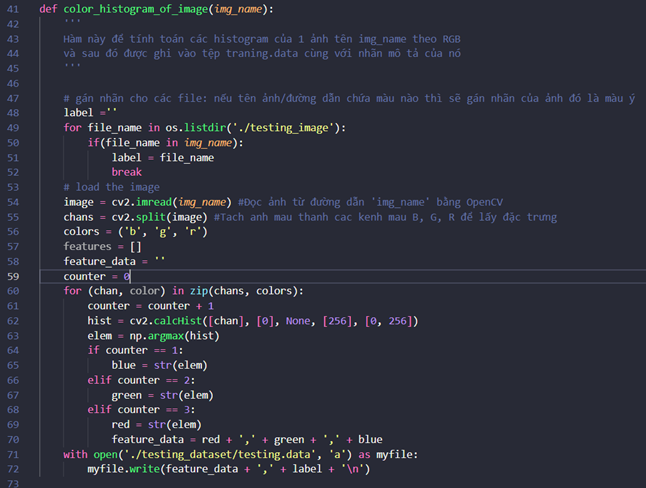
\includegraphics[scale=0.85]{BTL BaoCao Latex TTNT/Anh/trích xuất đặc trưng của file training.png}
    \captionsetup{justification=centering}
    \caption{Trích xuất đặc trưng của mẫu dữ liệu Training}
    \label{fig:train_data}
\end{figure}
Lần lượt duyệt qua từng tệp ảnh và lưu nó vào file testing.data để sử dụng trong quá trình đánh giá mô hình. Cài đặt được mô tả cụ thể như hình \ref{fig:data_label}
\begin{figure}[H]
    \centering
    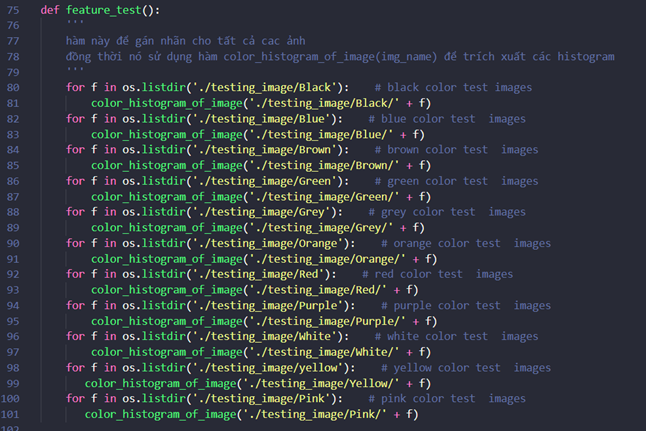
\includegraphics[scale = 0.85]{BTL BaoCao Latex TTNT/Anh/tiền xử lý.png}
    \caption{Tạo vector đặc trưng và nhãn của tệp ảnh}
    \label{fig:data_label}
\end{figure}
\subsubsection{Đối với mẫu dữ liệu Predict}
Mẫu dữ liệu Predict khác mẫu dữ liệu trong tập Training/Test ở chỗ nó không có nhãn, bởi vậy nhóm em đề xuất hàm color\_histogram\_of\_test\_image với chức năng và cách làm tương tự hàm color\_histogram\_of\_imag, tuy nhiên được bỏ đi phần gán nhãn. Cụ thể trong hình \ref{fig:test_data}
\begin{figure}[H]
    \centering
    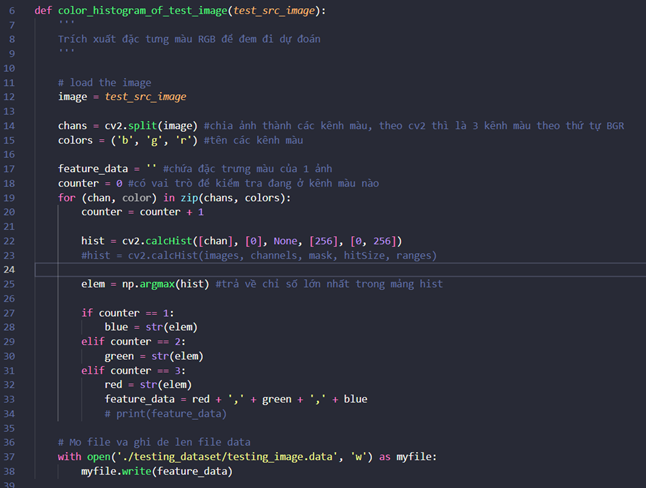
\includegraphics[scale=0.85]{BTL BaoCao Latex TTNT/Anh/trích xuất đặc trưng của file dự đoán.png}
    \captionsetup{justification=centering}
    \caption{Trích xuất đặc trưng của mẫu dữ liệu Predict}
    \label{fig:test_data}
\end{figure}

\section{Sử dụng phương pháp K-nearest Neighbors để phân loại màu ảnh}
\section{Đánh giá mô hình}
\section{Kết quả thu được}
\end{document}